\documentclass[10pt]{article}
\usepackage{amsmath, amsfonts, amssymb, amsthm}
\usepackage[colorlinks=true, allcolors=blue]{hyperref}
\usepackage{tikz}
\usepackage{xcolor}
\usepackage{pgfplots}

\begin{document}

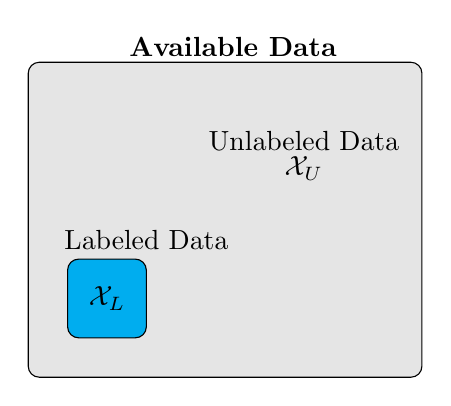
\begin{tikzpicture}
\draw[fill={gray!20}, rounded corners] (-2,-2) rectangle (3,2);
\node at (0.6, 2.2) {\textbf{Available Data}};

\draw[fill=cyan, rounded corners] (-1.5,-1.5) rectangle (-0.5,-0.5);
\node at (-1, -1) {$\mathcal{X}_L$};
\node[above] at (-0.5,-0.5) {Labeled Data};

\node at (1.5, 1) {Unlabeled Data};
\node at (1.5, 0.65) {$\mathcal{X}_U$};
    
\end{tikzpicture}

\end{document}